\chapter{REVISÃO DE LITERATURA}\label{CAP2}

\section{APRESENTAÇÃO DO TEMA}
O pavimento é uma estrutura de múltiplas camadas de espessuras finitas, construída sobre a superfície final de terraplenagem \cite{bernuccipavimentaccao}  e pode ser classificado  tradicionalmente em dois tipos básicos: rígidos e flexíveis. Os pavimentos podem ainda ser classificados como mistos, quando forem compostos pela combinação dos tipos citados anteriormente.  A utilização de um ou outro tipo depende de fatores como o clima da região, a função desempenhada e a carga à qual ele será submetido. Dentre as rodovias brasileiras, a maior parte é composta por pavimentos flexíveis (asfálticos), já os pavimentos aeroviários são em geral rígidos (concreto) ou mistos. 

A estrutura de um pavimento flexível é formada por quatro camadas principais: revestimento asfáltico, base, sub-base e reforço do subleito, sendo que uma ou mais camadas podem estar ausentes dependendo da intensidade do tráfego e dos materiais disponíveis. O revestimento é a camada superior e destina-se a resistir diretamente às ações do tráfego e transmiti-las de forma atenuada às camadas inferiores \cite{bernuccipavimentaccao}, desempenhando papel fundamental na estrutura da via. São as propriedades dos materiais de revestimento que irão definir aspectos importantes para os usuários, tais como: aderência entre o pneu e o pavimento, projeção de água de chuva, o desgaste dos pneus e o ruído no exterior e no interior do veículo. Portanto, é de fundamental importância quantificar essas propriedades e estudar maneiras de melhorar seu desempenho. 

As características dos agregados que compõem o asfalto exercem grande influência nas propriedades do pavimento. Por isso, identificar o tipo de agregado utilizado na mistura asfáltica é uma forma confiável de prever algumas características da superfície. \citeonline{bernuccipavimentaccao} descreve as composições granulométricas dos pavimentos de Concreto Asfáltico (CA), também denominados Concreto Betuminoso Usinado a Quente (CBUQ), a saber:
\begin{itemize}
\item Graduação densa: curva granulométrica contínua e bem-graduada de forma a proporcionar um esqueleto mineral com poucos vazios visto que os agregados de dimensões menores preechem os vazios dos maiores; 

\item Graduação aberta: curva granulométrica uniforme com agregados quase exclusivamente de um mesmo tamanho, de forma a proporcionar um esqueleto mineral com muitos vazios interconectados, com insuficiência de material fino (menor que 0,075mm) para preencher os vazios entre as partículas maiores. Tem o objetivo de tornar a mistura com elevado volume de vazios com ar e, portanto, drenante, possibilitando a percolação de água no interior da mistura asfáltica. Exemplo: mistura asfáltica drenante, conhecida no Brasil por Camada Porosa de Atrito (CPA); 

\item Graduação descontínua: curva granulométrica com proporcionamento dos grãos de maiores dimensões em quantidade dominante em relação aos grãos de dimensões intermediárias, completados por certa quantidade de finos, de forma a ter uma curva descontínua em certas peneiras(...). Exemplo: Matriz Pétrea Asfáltica (Stone Matrix Asphalt – SMA); mistura sem agregados de certa graduação (gap-graded). 
\end{itemize}

\section{CONCEITOS BÁSICOS}
Com o objetivo de melhor viabilizar o entendimento das propriedades do revestimento asfáltico e do método de avaliação de pavimento proposto, faz-se necessária a apresentação e distinção de alguns conceitos específicos que surgem na literatura.

\subsection{Textura superficial}

A EN ISO 113473-1:1997 \nocite{iso113473} apresenta a seguinte definição de textura de um pavimento:  “Desvio entre uma superfície de um pavimento e uma superfície completamente plana de referência dentro dos limites das escalas de comprimento de ondas definidos [...]”; tradução livre. 
\apudonline {dagnall}{machado}
afirma que a textura superficial é: “Um conjunto de irregularidades, isto é, pequenas saliências e reentrâncias que caracterizam uma superfície”.
Entende-se, portanto, que a textura corresponde a qualquer tipo de desvio na superfície do pavimento, podendo ocorrer em maior ou menor escala. \citeonline{wambold} classifica os níveis de textura em:

\begin{itemize}
\item Microtextura: corresponde às rugosidades, cujos comprimentos de onda
variam entre 0 a 0,5mm e amplitude de 0 a 0,2mm. Está relacionada à própria superfície do agregado mineral e faz o pavimento parecer mais ou menos áspero, sendo muito pequena para ser percebida a olho nu;

\item Macrotextura: corresponde às rugosidades com comprimento de onda de 0,5 a 50mm e amplitude de 0,2 a 10mm. Representa as asperezas superficiais do pavimento causadas pelas protuberâncias do agregado, é da ordem de grandeza da área de contato pneu/pavimento;

\item Megatextura: corresponde às rugosidades cujos comprimentos de onda variam entre 50 e 500mm e amplitude entre 10 a 500mm. Essa textura é da mesma ordem de grandeza dos pneus e implica em falhas no pavimento;

\item Irregularidade: corresponde a desvios maiores que 500mm, com comprimentos de onda superiores a 500mm. A irregularidade é uma ocorrência indesejável.
\end{itemize}

Os quatro níveis de textura identificados acima estão representados na Figura \ref{Fig:tipos_textura}, abaixo:

\begin{figure}[!ht]
\centering
\caption{Representação das quatro categorias de textura.} 
{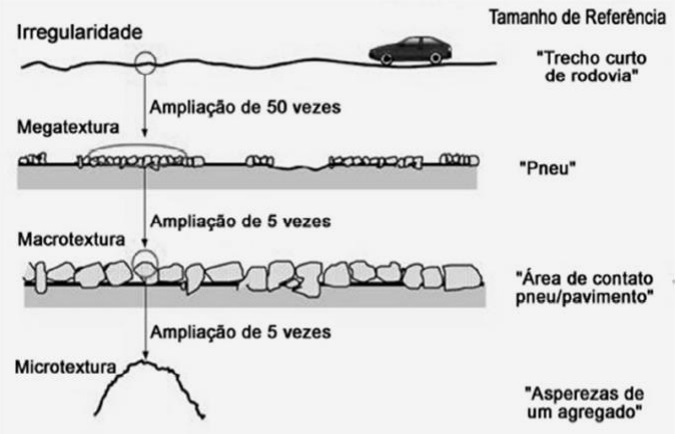
\includegraphics[scale=.70]{figures/tipos_textura.jpg}}\\
\makebox[\width]{Fonte: baseado em \citeonline{kuchiishi}} \label{Fig:tipos_textura}
\end{figure}

\subsection{Rugosidade}
\citeonline{piratelli} define o conceito de rugosidade como o  conjunto de desvios microgeométricos caracterizado pelas pequenas saliências e reentrâncias presentes em uma superfície. Para \apudonline{scheers}{machado} a rugosidade é o conjunto de oscilações de alta freqüência ou de ondas curtas.

Há uma grande similaridade entre as definições de rugosidade e textura, que por vezes chegam a se confundir. Entendemos aqui, a rugosidade como a ocorrência de desvios na superfície e textura como o efeito causado por esses desvios. Os diferentes níveis de rugosidade, corresponderiam portanto, aos diferentes níveis de textura descritos anteriormente, quando os desvios são de ordem de grandezas maiores, caracterizam ondulação e erro de forma (Figura \ref{Fig:rugosidade}). 

\begin{figure}[!ht]
\centering
\caption{Representação dos diferentes níveis de rugosidade.}
{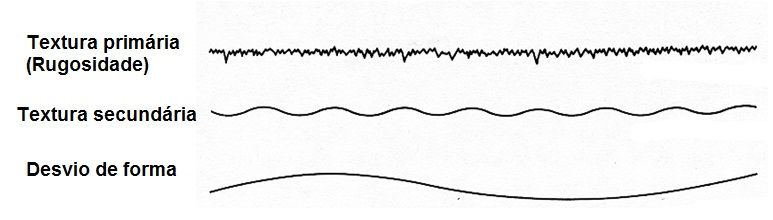
\includegraphics[scale=.70]{figures/rugosidade.jpg}}\\
\makebox[\width] {Fonte: \citeonline{piratelli}} \label{Fig:rugosidade}
\end{figure}

A diferença entre rugosidade, ondulação e erro de forma é baseada no comprimento de onda da superfície analisada ou no espaçamento entre picos \apud{demare}{machado} porém a fronteira entre rugosidade e ondulação é questionável e deve-se especificar numericamente o comprimento da frequência de onda acima ou abaixo do qual uma das componentes da superfície (rugosidade ou ondulação) é eliminada \cite{machado}. 

\subsection{Superfície}
A superfície real de um objeto é definida pela NBR ISO 4287:2002 \nocite{iso4287} como a superfície que limita o corpo e o separa do meio ambiente, ela pode ser representada pela superfície efetiva que é aquela obtida por meio das técnicas de medição. Estes conceitos estão representados na Figura \ref{Fig:superficie}.

\begin{figure}[!ht]
\centering
\caption{Representação das superfícies real e efetiva.} 
{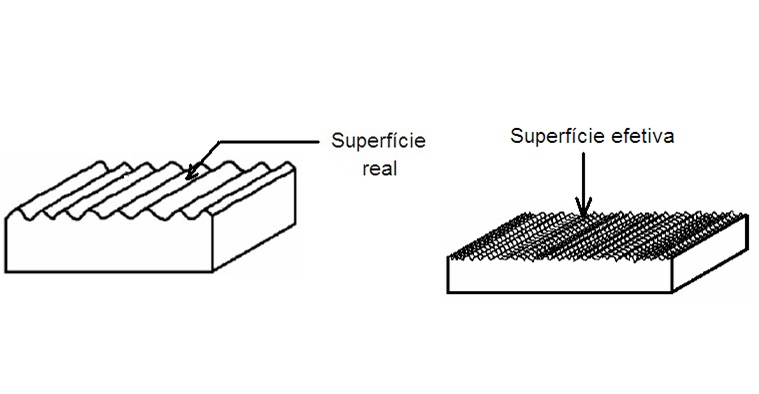
\includegraphics[scale=.65]{figures/superficie.jpg}}\\
\makebox[\width]{Fonte:Adaptado de \citeonline{piratelli}} \label{Fig:superficie}
\end{figure}

\subsection{Perfil de Superfície}
O perfil de superfície é uma representação bidimensional geralmente orientada em um eixo x-y. Ele é resultante da interseção da superfície real e um plano específico NBR ISO 4287:2002 \nocite{iso4287}, como representado na Figura \ref{Fig:perfil_de_superficie}.

\begin{figure}[!ht]
\centering
\caption{Obtenção do perfil de superfície.}
{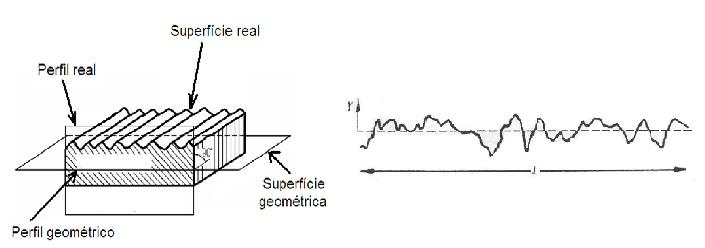
\includegraphics[scale=0.84]{figures/perfil_de_superficie.jpg}}\\
\makebox[\width]{Fonte: Adaptado de \citeonline{piratelli}} \label{Fig:perfil_de_superficie}
\end{figure}

Na prática é usual escolher um plano onde a normal é teoricamente paralela à superfície real e em uma direção apropriada (NBR ISO 4287:2002\nocite{iso4287}).

Para obtenção de um perfil que represente a superfície efetiva existem vários ensaios e equipamentos, contudo alguns métodos como os perfilométricos acabam gerando um perfil composto por todos os níveis de textura, o que nem sempre é prático para a análise que se deseja realizar. Para permitir a separação entre os perfis de rugosidade e de ondulação, a norma propõe uma correção que consiste na filtragem do perfil primário. Assim, temos que a definição do perfil de rugosidade é a seguinte: "perfil derivado do perfil primário pela eliminação dos componentes de comprimento de ondas longas, usando o filtro de perfil $\lambda$c” (NBR ISO 4287:2002). No presente trabalho, esta correção não se fez necessária, uma vez que as dimensões dos corpos de prova utilizados são pequenas, assim os desvios no nível das ondulações e desvios de forma não foram representados.

A partir dos perfis medidos podem ser realizadas caracterizações de parâmetros superficiais específicos \cite{machado}, alguns elementos do perfil devem ser analisados para que se obtenham estes parâmetros. A seguir estão apresentadas as definições compiladas a partir das normas EN ISO 113473-1:1997 \nocite{iso113473} e NBR ISO 4287:2002 \nocite{iso4287}, foram ainda acrescidas as definições de outros autores quando necessário.

\subsection{Linha Média (LM)} 
De acordo com \citeonline{machado} a linha média, identificada na Figura \ref{Fig:lm_e_ca} pode ser determinada de duas maneiras: linha média dos mínimos quadrados, referente ao perfil primário; e linha média filtrada, referente aos perfis de rugosidade e de ondulação.

A primeira definição é apresentada pela NBR ISO 4287:2002\nocite{iso4287}, que define a linha média do perfil como a linha determinada pelo ajuste dos mínimos quadrados à linha da forma nominal do perfil. Ou seja, essa linha acompanha o perfil nominal, de forma que a soma dos quadrados dos desvios do perfil na direção vertical seja minimizado.

A definição da linha média filtrada consta no trabalho de \citeonline{piratelli}, segundo a qual a linha média divide o perfil tal que a soma das áreas acima é igual à soma das áreas abaixo, ao longo do comprimento de medição.

\subsection{Comprimento de Amostragem (L)}
O comprimento de amostragem está identificado na Figura \ref{Fig:lm_e_ca}, a norma o define como sendo o comprimento na direção do eixo X, usado para identificar as irregularidades características do perfil sob avaliação; ou seja, é o comprimento do trecho a ser avaliado.

\begin{figure}[!ht]
\centering
{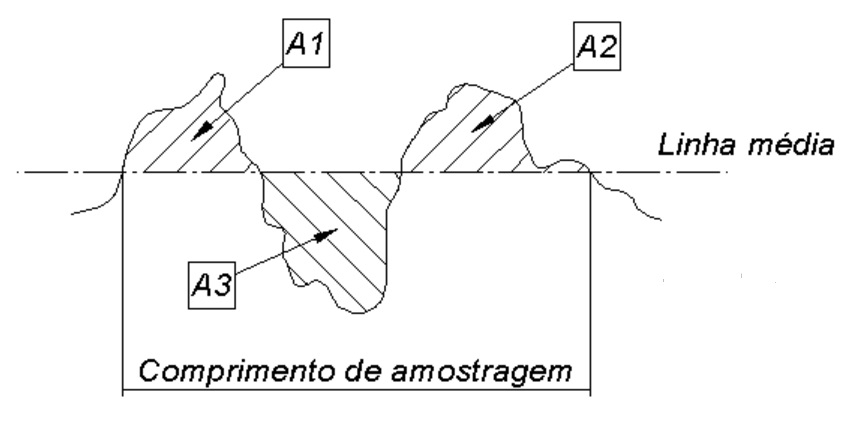
\includegraphics[scale=0.50]{figures/lm_e_ca.jpg}}\\\caption{Representação da linha média e do comprimento de amostragem.}
\makebox[\width]{Fonte: \citeonline{unicamp}} \label{Fig:lm_e_ca}
\end{figure}

\subsection{Altura de pico (Zp) e profundidade do vale (Zv)}
São respectivamente as distância verticais entre o eixo x e o ponto mais alto dos picos do perfil e entre o eixo x e o ponto mais baixo dos vales do perfil. A soma da altura do pico e profundidade do vale é denominada altura de um elemento do perfil (Zt), como representado na Figura \ref{Fig:alturas}.
 Conforme \citeonline{machado}, a avaliação dos picos é importante quando se consideram as propriedades de fricção e desgaste e a interação entre concentração de superfícies.

\begin{figure}[!ht]
\centering
{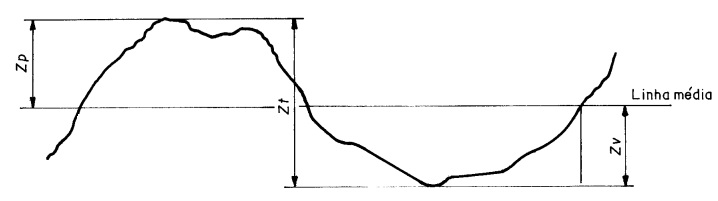
\includegraphics[scale=0.65]{figures/alturas.jpg}}\\\caption{Representação da altura de pico e profundidade de vale.}
\makebox[\width]{Fonte: Adaptado de NBR ISO 4287:2002 \nocite{iso4287}} \label{Fig:alturas}
\end{figure}

\subsection{Altura máxima do pico (Rp) e profundidade máxima de vale do perfil (Rv)}
Os parâmetros de amplitude máxima de picos e vales correspondem ao valor de maior altura de pico (Zp) e de maior profundidade de vale (Zv), no comprimento de amostragem. 
O somatório do mais alto pico (Rp) com o mais profundo vale (Rv) é chamado de amplitude de perfil (Rt). 

\subsection{Rugosidade média ou Amplitude média (Ra)}
O parâmetro de amplitude média de perfil, também é conhecido como média aritmética, média da linha central ou desvio médio aritmético do perfil.
É o valor médio das alturas dos elementos do perfil (Zt) no comprimento de amostragem, obtido pela Equação (\ref{Eq:rugosidademedia}).

\begin{equation}\label{Eq:rugosidademedia}
%
Ra = \frac{\sum Ai}{L}
%
\end{equation}
%

As variáveis $Ai$, $L$ representam respectivamente a área sob a curva entre dois pontos nulos e o comprimento de amostragem, como indicado na Figura \ref{Fig:lm_e_ca}. 

De acordo com \citeonline{machado}, este parâmetro corresponde à área entre o perfil de rugosidade e a linha média, ou ainda, a integral dos valores absolutos das amplitudes do perfil de rugosidade dentro de um comprimento de amostragem.

\subsection{Textura Média do Perfil (MPD)}
É o valor médio da rugosidade do perfil dentro de um comprimento de amostragem. 
Diferença entre a média aritmética de dois picos ($Z_1$ e $Z_2$) e a linha média (LM)\footnote{Observe que a Linha Média não corresponde necessariamente ao eixo coordenado x, quando isso ocorre, o valor de LM na equação é zero.}  em uma distância de 100m. Este parâmetro é obtido pela Equação \ref{Eq:texturamedia}: 

\begin{equation}\label{Eq:texturamedia}
%
MPD = \frac{Z_{1}+Z_{2}}{L} - LM 
%
\end{equation}
%

\section{PARÂMETROS ESTATÍSTICOS
}
O algoritmo utilizado, além de retornar a medida da rugosidade média  e o erro percentual em relação aos dados experimentais, também calcula alguns parâmetros estatísticos descritivos como Desvio padrão, Mediana e Curtose. Estes parâmetros possibilitam a análise quantitativa dos dados.

\subsection{Desvio Médio Quadrático (Rms)}
É uma medida gerada a partir do Desvio Padrão, fornece informações referentes à dispersão dos dados, permitindo analisar  como as alturas se comportam quando distantes da média. É definido como a raiz quadrada da média dos valores das ordenadas $Z(x)$, oferecendo uma medida do desvio padrão dos dados analisados. Este parâmetro é obtido pela Equação \ref{Eq:rms}.

\begin{equation}\label{Eq:rms}
%
Rms = \sqrt\frac{1}{l} \int_0^l Z^2(x)  dx
%
\end{equation}
%

\subsection{Fator de achatamento ou Curtose (Rku)}

A curtose indica a facilidade de se obter valores que não se aproximam da média, representando que a distribuição dos resultados tem achatamento semelhante ao da distribuição normal quando esta medida de dispersão se aproxima de zero \cite{magalhaes}. É definida como o quociente entre o valor médio dos valores das ordenadas Z(x) à quarta potência e o valor de Rms à quarta potência. Este parâmetro é obtido pela Equação \ref{Eq:rku}.

\begin{equation}\label{Eq:rku}
%
Rku = \frac{1}{Rms^4} \bigg[\sqrt\frac{1}{l} \int_0^l Z^4(x)  dx \bigg] 
%
\end{equation}
%

Como enfatizado na NBR ISO 4287:2002\nocite{iso4287}, a curtose é um parâmetro fortemente influenciado por picos isolados ou vales isolados. \citeonline{bernuccipavimentaccao} destaca que, em pavimentos asfálticos, as alturas das asperezas podem não ser normalmente distribuídas, apresentando assim valores distintos de Rku, o que faz com que as superfícies do pavimentos apresentem 
configurações variadas, como mostra a Figura \ref{Fig:curtose}.

\begin{figure}[!ht]
\centering
{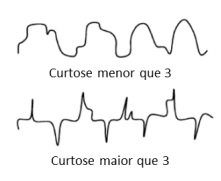
\includegraphics[scale=1.1]{figures/curtose.jpg}}\\
\caption{Influência da curtose na no perfil de superfície.} \makebox[\width]{Fonte:\citeonline{bernuccipavimentaccao}} \label{Fig:curtose}
\end{figure}


\subsection{Mediana (Md)}
A mediana é o valor central de um conjunto de dados, dividindo-o em duas partes iguais. É um parâmetro menos sensível a valores atípicos. Este parâmetro é obtido pela Equação \ref{Eq:md}.

\begin{equation}\label{Eq:md}
%
Md = L_i+\bigg(\frac{\frac{n}{2}-\sum{f'}}{f_{Md}}\bigg) C_{Md}
%
\end{equation}
%

Onde $L_i$ é o limite inferior da classe mediana; $n$ é o total
de frequência; $\sum{f’}$ é soma de todas as frequências das classes inferiores à mediana, $f_{Md}$ é a frequência da classe mediana e $C_{Md}$ é a amplitude da classe mediana.


\section{INFLUÊNCIA DA RUGOSIDADE NO DESEMPENHO DE PAVIMENTOS}
Os desvios na superfície do pavimento são de fundamental importância para garantir condições de segurança e conforto nas rodovias. Para avaliar o estado de conservação dos pavimentos, diversos indicadores foram desenvolvidos ao longo dos anos. O Instituto de Infra-Estruturas Rodoviárias (INIR), em sua disposição técnica \citeonline{azevedo} cita parâmetros de avaliação das características superficiais e estruturais, baseados na rugosidade. São eles:
\begin{itemize}
\item Textura Superficial;
\item Irregularidade Longitudinal;
\item Perfil Transversal. 
\end{itemize}

Cada nível de textura está relacionado à uma propriedade física do pavimento. O atrito no clima seco, por exemplo, é influenciado pelos níveis de macrotextura e microtextura, ou seja, por rugosidades compreendidas no intervalo  entre 1$\mu$m e 10mm, como representado na Figura \ref{Fig:influencia}.


\begin{figure}[!ht]
\centering
{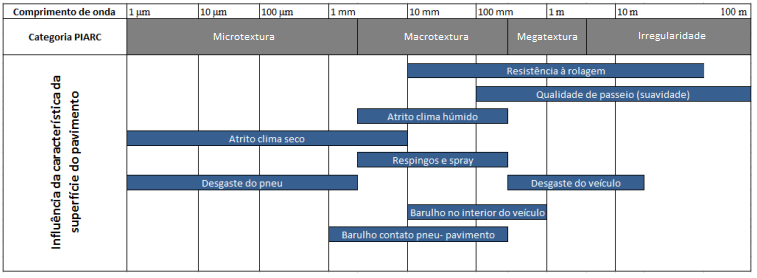
\includegraphics[scale=0.8]{figures/influencia.jpg}}\\
\caption{Influência das características da superfície no desempenho dos pavimentos.} 
\makebox[\width]{Fonte: \citeonline{bitelli}} \label{Fig:influencia}
\end{figure}

A macrotextura garante a resistência à derrapagem, principalmente em velocidades elevadas ou quando o pavimento encontra-se molhado, contribui também para melhorar a visibilidade em condições de pista molhada, elimina ou atenua a reflexão da luz melhorando a percepção das marcas de sinalização horizontal e reduz o barulho gerado pelo contato entre pneu e pavimento. A microtextura, ou a aspereza do pavimento, por sua vez, é necessária para se conseguir uma boa aderência a baixas velocidades e no pavimento seco, além de regular o desgaste dos pneus.

A megatextura e a irregularidade superficial são características indesejáveis, de qualquer ponto de vista. Incidem negativamente sobre o conforto e aumentam o ruído de rolamento, os gastos com a manutenção dos veículos e os gastos com a conservação do pavimento \cite{azevedo}.

Observa-se que os níveis que predominantemente afetam o atrito são a microtextura e a macrotextura, por isso, essas características são os principais objetos de estudos que relacionam a rugosidade e o desempenho de pavimentos. Dentre eles podemos citar o de \citeonline{boscaino}, que correlacionou propriedades de superfícies asfálticas, como a textura superficial, com a absorção acústica dos pavimentos. O mesmo tema foi abordado por \citeonline{callai}, que realizou um estudo de caso na cidade de São Paulo, analisando a emissão de ruído em diferentes tipos de revestimento. 

Outro estudo de caso foi conduzido por \citeonline{pulugurtha} na Carolina do Norte, Estados Unidos. Ele associou o efeito da macrotextura com o aumento da segurança da pista, provando uma forte relação entre ambos. No Brasil, estudos semelhantes foram desenvolvidos, como o de \citeonline{dasilva}, em São Paulo, o qual avaliou a redução de acidentes na rodovia Fernão Dias com a troca do revestimento da pista. Os resultados demonstraram que após a substituição do Concreto Asfáltico, que apresenta uma textura fina, pelo Microrrevestimento cuja textura varia de média a grossa, houve uma significativa redução dos acidentes.  

Segundo \citeonline{bitelli}, os indicadores de performance são, em geral, relacionados às diferentes condições de medição (velocidade de deslizamento, estado da superfície, ângulo entre as direções de deslocamento e os pneus, etc.), cada uma possui uma ténica de medição específica, geralmente regulmentada por padrões nacionais ou internacionais. Dentre os ensaios e aparelhos criados para aferição dos parâmetros superficias de um pavimento, classificam-se os métodos em perfilométricos ou estáticos. 

Nas medições estáticas, destaca-se o Ensaio de Mancha de Areia, que mede a rugosidade em nível de macrotextura. A eficiência deste ensaio foi objeto de pesquisa como \citeonline{specht} e  \citeonline{kuchiishi}. Outro ensaio é o chamado Pêndulo Britânico, destinado à medição da rugosidade à nível da microtextura como estudado por \citeonline{lee}. Há ainda pesquisas que utilizam processamento de imagens como método de caracterização da textura \cite{slimane}, \cite{khoudeirs}.

Em relação aos métodos perfilométricos há diversos tipos de equipamentos disponíveis. No nosso país, os equipamentos empregados em maior escala são os do tipo resposta, que fornecem um somatório de desvios do eixo de um veículo em relação à suspensão ou até mesmo por meio de levantamentos topográficos. Um destes aparelhos é o chamado rugosímetro BPR, porém ele apresentou falhas como indicado por \citeonline{perera}, uma vez que estava sujeito à variações de temperatura além de produzir algumas frequências resssoantes que provocaram resultados incorretos. O   Maysmeter, foi outro equipamento amplamente utilizado entre os anos de 1960 e 1980, inclusive no Brasil, pelo antigo DNER (Departamento Nacional de Estradas de Rodagem). Contudo, este acabou sendo substituído no país pelo perfilômetro inercial desenvolvido em parceria pelo IPR (Instituto de Pesquisas Rodoviárias) e pela USP (Universidade de São Paulo). Este equipamento consiste em um veículo de passeio no qual são acoplados um sensor de deslocamentos verticais e um quantificador de irregularidade, o desenvolvimento e utilização deste equipamento foi descrito por \citeonline{barella}. 

\section{EMPREGO DE MÉTODOS DE ESCANEAMENTO PARA ANÁLISE DE PAVIMENTO}

Nos últimos anos, os dispositivos de escaneamento a laser têm sido difundidos e se tornado mais acessíveis, assim, diversas aplicações para este equipamento vem sendo estudadas. O sistema de escaneamento com uso de laser é um dos tipos de técnicas denominadas LiDAR (Light Detection and Ranging). Nesta classificação podemos discernir ainda os escaneamentos dos tipos ALS, TLS e MLS, respectivamente: escaneamento aéreo a laser, escaneamento terrestre a laser e escaneamento móvel a laser, em tradução livre. Dentre os usos já explorados para essa tecnologia, podemos citar estudos nas áreas de: gerenciamento florestal \cite{means}, \cite{giongo}, mapeamento de regiões \cite{schwarz} e na indústria automotiva \cite{rasshofer}.

A caracterização da textura superficial de pavimentos por meio de escaneamento tridimensional conforme proposto neste trabalho, já foi realizada por outros autores como \citeonline{bitelli}, cujo procedimento foi uma das referências para esta pesquisa. Ressalta-se dentre as similaridades, o uso de corpos de prova extraídos em campo, além de outros moldados in-loco e também o uso do mesmo equipamento, o Next Engine® laser scanner.  Os parâmetros obtidos foram agrupados em duas classes: a primeira leva em consideração parâmetros “geométricos” relacionados à morfologia da amostra analisada; a segunda classe inclui indicadores estatísticos do desempenho(...), que analisam os aspectos da interação entre o pneu e a superfície do pavimento \cite{bitelli}.

A conclusão do experimento de \citeonline{bitelli} foi bastante satisfatória, a análise dos diferentes tipos de pavimento: DGAC (concreto asfáltico de graduação densa); SMA (concreto asfalto de graduação descontínua), e OGAC (concreto asfáltico de graduação aberta); correspondeu às expectativas, caracterizando o DGAC como um pavimento menos rugoso e o OGAC como o de maior rugosidade.

\citeonline{sengoz} utilizaram o scanner Metris Model Maker D100 3D e comapararam os resultados com o tradicional ensaio de Mancha de Areia. O equipamento utilizado foi montado sobre uma base móvel e conectado à um computador para realizar a coleta de dados. Para análise dos resultados, foi traçada uma curva MPD (profundidade média do perfil) versus MTD (profundidade média da textura) e foi encontrado o coeficiente de correlação bastante elevado de $R^2 = 0.97$. Baseando-se nas conclusões da PIARC (congresso internacional sobre rodovias, produzido pela \emph{World Road Association}) de que o melhor parâmetros para determinação do coeficiente de atrito seria o MPD,  eles verificam que o a o partir do MTD pode-se também prever de forma satisfatória este coeficiente.

\citeonline{pratico} conduziram outro estudo focado na relação entre no MPD e no MTD. Porém, este utilizou um equipamento de escaneamento bidimensional. Foram considerados os seguintes tipos de revestimentos: DGFC (revestimento de graduação densa), SMA (revestimento de graduação descontínua), OGFC (revestimento de graduação aberta) e PEM (mistura porosa). Verificou-se que para rugosidades inferiores a 1,5mm, uma função linear era bem representativa. Contudo, para valores acima de 1,5mm, houve uma visível divergência de resultados. O estudo concluiu que a correlação entre o MPT e a medida do ensaio de mancha de areia apresenta algumas complexidades e que a divergência encontrada baseia-se essencialmente no fato de que o ensaio é tridimensional, enquanto o escaneamento realizado era bidimensional. Para associar os resultados, foi adaptada uma curva e apesar das ressalvas, a conclusão deste estudo foi um modelo satisfatório para correlacionar as grandezas, e que representa uma boa parte dos pavimentos asfaltos em uso.

\citeonline{celko} em sua pesquisa, medem a macrotextura e realizam uma comparação minuciosa entre medições feitas a partir do Método Volumétrico (MTD) e do perfilômetro GE (MPD) com medições do ZScanner\textsuperscript{\textregistered} 800, também é feita a medição e comparação do coeficiente de atrito por diferentes métodos. As medições obtidas pelo scanner são processadas por meio de um algoritmo desenvolvido no MATLAB\textsuperscript{\textregistered}. É interessante ressaltar que em todas as comparações foram obtidos resultados razoalmente próximos, principalmente, entre os valores do scanner 3D e do método volumétrico, para a qual foi obtido o coeficiente de correlação $R^2 = 0.94$. A diferença entre o método aqui apresentado e o proposto por \citeonline {celko} consiste principalmente no fato de que o foi utilizado um scanner fixo, sendo necessária a extração de amostras para que fosse possível realizar o escaneamento. Ainda assim, espera-se que seja possível comparar os resultados como forma de validação do método.  

